%% 
%% Copyright 2019 Elsevier Ltd
%% 
%%
%%%%%%%%%%%%%%%%%%%%%%%%%%%% ! ! ! SUBMISSION CHECKLIST ! ! ! %%%%%%%%%%%%%%%%%%%%%%%%%%%%
%%
%% Please confirm that your submission follows all the requirements of the guidelines, including the submission checklist:
%% _ Cover letter
%% _ Highlights
%% _ Authorship statement
%% _ The manuscript must be single column and double spaced
%% _ Reference must be in the author-date format
%% _ Code availability section 
%%
%% *All the manuscripts in disagreement with the guidelines will be desk-rejected without editorial check.
%%
%% --------------------------------------
%%
%% This file is part of the 'CAS Bundle'.
%%  
%% It may be distributed under the conditions of the LaTeX Project Public
%% License, either version 1.2 of this license or (at your option) any
%% later version.  The latest version of this license is in 
%%    http://www.latex-project.org/lppl.txt 
%% and version 1.2 or later is part of all distributions of LaTeX
%% version 1999/12/01 or later.
%%   
%% The list of all files belonging to the 'CAS Bundle' is
%% given in the file `manifest.txt'.
%% 
%% Template article for cas-dc documentclass for  
%% double column output.
 
%\documentclass[a4paper,fleqn,longmktitle]{cas-dc}
\documentclass[a4paper,fleqn]{cas-sc}

\usepackage[authoryear]{natbib}
\usepackage{graphicx} 
\usepackage{float}
\usepackage{algorithm}  
\usepackage{algpseudocode}
\usepackage{color}
\usepackage{setspace}
\usepackage[nomarkers,figuresonly]{endfloat}


\newcommand{\colorComments}{black} 
 
%%%Author definitions
\def\tsc#1{\csdef{#1}{\textsc{\lowercase{#1}}\xspace}}
\tsc{WGM}
\tsc{QE}
\tsc{EP}
\tsc{PMS}
\tsc{BEC}
\tsc{DE}
%%%

\usepackage{lineno}
\linenumbers 

\begin{document}
\let\WriteBookmarks\relax
\def\floatpagepagefraction{1}
\def\textpagefraction{.001}
\shorttitle{Comparison of deep learning and ensemble learning methods in slope-unit-based landslide susceptibility prediction}
\shortauthors{Yingxu Song et al}

\title [mode = title]{Comparison of deep learning and ensemble learning methods in slope-unit-based landslide susceptibility prediction}



\author[1]{Yingxu Song} [type=editor,
auid=000,bioid=1,orcid=0000-0002-9273-2019]
\credit{Conceptualization, Methodology, Software, Validation, Investigation, Resources, Funding acquisition}

\author[2]{Huijuan Zhang}[]
\credit{Conceptualization, Validation, Writing-original draft preparation, Writing-review and editing}

\author[3]{Zhiwen Li}
\credit{Conceptualization}

\author[4]{Shiluo Xu}
\credit{Software, Resources}

\author[5]{Yueshun He}
\credit{Project administration, Funding acquisition}

\author[7]{Xianyu Yu}
\credit{Resources, Funding acquisition}

\author[8]{Ye Liang}
\credit{Funding acquisition}

\author[1]{Weicheng Wu}
\credit{Writing-review and editing}

\author[2]{Yue Wang}
\credit{Software}

\address[1]{School of Earth Sciences, East China University of Technology, Nanchang, Jiangxi Province 330013, China}
\address[2]{Key Lab of Digital Land and Resources and Faculty of Earth Sciences, East China University of Technology, Nanchang, 330013, Jiangxi, China}
\address[3]{Jiangxi Engineering Laboratory on Radioactive Geoscience and Big Data Technology, School of Information and Engineering, East China University of Technology, Nanchang, 330013, Jiangxi, China; yxsong@ecut.edu.cn}
\address[4]{School of Information Engineering, Huzhou University, Huzhou 313000, China; xushiluo@163.com} 
\address[5]{East China University of Technology, Nanchang, 330013, Jiangxi, China; heys@ecut.edu.cn} 
\address[6]{School of Environmental and Chemical Engineering, Foshan University, Foshan, 528000, China; lizw1982@163.com} 
\address[7]{School of Civil Engineering, Architecture and Environment, Hubei University of Technology, Wuhan, Hubei Province 430074, China; yuxianyu@hbut.edu.cn} 
\address[8]{Jiangxi Engineering Technology Research Center of Nuclear Geoscience Data Science and System, East China University of Technology, Nanchang, 330013, Jiangxi, China; liangye@ecut.edu.cn} 
\address[1]{Key Lab of Digital Land and Resources and Faculty of Earth Sciences, East China University of Technology, Nanchang, 330013, Jiangxi, China; wuwch@ecut.edu.cn/wuwc030903@sina.com} 
\address[2]{School of Earth Sciences, East China University of Technology, Nanchang, Jiangxi Province 330013, China; 2020210058@ecut.edu.cn} 


\begin{abstract}
In this article, we discussed the applicability of deep learning methods and ensemble learning methods in slope-unit-based landslide susceptibility prediction (LSP).
For this purpose, we presents a case study in Wanzhou section of the Three Gorges Reservoir area, China, and chooses slope units as the basic mapping units.
Three deep learning models, that is long short-term memory (LSTM), recurrent neural network (RNN), and gate recurrent unit (GRU), and a ensemble learning model (LightGBM) were used to carry out LSP.
Firstly, 29 landslide factors and 1,909 slope unit generated from a digital elevation model (DEM) were selected as the input data of the study.
Of the 1,909 slope units in the inventory, 40\% were used for validation, and the remaining 60\% were used for training purposes. 
Then, LSP was carried out using the above five models, respectively.
Next, the area under the curve (AUC) and landslide prediction index (LPI) were used to validate performance and accuracy of the models.
In each landslide susceptibility map, the LPI were classed as having very high landslide susceptibility, followed by the high, moderate, low and very low landslide susceptibility classes, respectively.
Unexpectedly, the performance of deep learning models is weaker than ensemble learning models. 
The AUC of the LSTM, RNN, GRU and LightGBM is 0.723, 0.731, 0.762, 0.915, respectively. 
Therefore, the deep learning model is not applicable in this situation, which also provides a new perspective for the prediction of landslide susceptibility in other regions.
\end{abstract}
 
\begin{coverletter}

Dear Editors-in-Chief,
\newline

please find the enclosed manuscript "Comparison of deep learning and ensemble learning methods in landslide susceptibility prediction " which we are submitting for exclusive consideration for publication in Computers \& Geosciences. 
We confirm that the submission follows all the requirements and includes all the items of the submission checklist.  
\newline

In this contribution, to solve the imbalanced landslide samples (landslides, non-landslides) in the landslide susceptibility evaluation, the application of the class-weighted algorithm combined with traditional machine learning (logistic regression) and ensemble machine learning models (LightGBM and random forest) have been investigated. 
Wanzhou section of the Three Gorges Reservoir area, China, where the number of landslide samples is 19 times more than non-landslide samples, is chosen as an example. 
The landslide inventory database was produced using field investigation and remote sensing images provided by Google Earth. Of the 233 landslides in the inventory, 40\% were used for validation, and the remaining 60\% were used for training purposes. Twelve environmental parameters (elevation, slope, aspect, curvature, distance to river, NDVI, NDWI, rainfall, seismic intensity, land use, TRI, lithology) were used as inputs of the models to produce landslide susceptibility map (LSM). 
The AUC value, Balanced accuracy, and Geometric mean score were used to estimate the quality of models. 
Research has found that the weighted models (weighted logistic regression, weighted LightGBM, weighted random forest) are better than unweighted methods and the weighted random forest method has the best performance. 
The class-weighted algorithm turned the susceptibility evaluation problem into a cost-sensitive problem by setting unequal weights for different classes, which is probably to be applied to the landslide susceptibility evaluation in other areas.
\newline

We provide the source codes in a public repository with details listed in the section "Code availability".
\newline

Thanks for your consideration. 
\newline
Sincerely,
\newline

Huijuan Zhang
\newline
Jiangxi Engineering Laboratory on Radioactive Geoscience and Big Data Technology, School of Information and Engineering, East China University of Technology, Nanchang, 330013, Jiangxi, China; yxsong@ecut.edu.cn
\end{coverletter}

 
\begin{highlights}
\item This study shows that deep learning methods worse than ensemble learning methods, which has certain enlightenment significance for the selection of methods in the evaluation of landslide susceptibility when the landslide samples are not enough.
\item The AutoML tools were used to train the best ensemble machine learning model, which could reduce unnecessary manual operations, and the LightGBM method was better than the others.
\item The ensemble models are much more applicable for slope-unit-based landslide susceptibility prediction than deep learning models.
\end{highlights}

\begin{keywords}
landslide susceptibility prediction\sep deep learning \sep slope-unit-based \sep ensemble learning \sep Three Gorges Reservoir area
\end{keywords}

\maketitle 

\printcredits

\doublespacing

\section{Introduction}
Landslide is one of the major geological hazards, which often causes heavy damage, leading to huge economic losses and casualties. 
landslide susceptibility prediction (LSP) is widely used in the management of landslide disasters to answer the question of "where" the landslide might occur \citep{pourghasemi2018analysis}. 
By combining geomorphologic conditions (slope, aspect, landcover, etc.) and dynamic factors (rainfall, earthquake, etc.) , LSP can be regarded as a binary classification problem \citep{Song2018, Khan2021}. 
Therefore, a large number of statistical methods and machine learning methods have been introduced into LSP, such as imformation value \citep{chen2016comparison_LSM_INFORVALUE, Gao2006IV_Wanzhou}, analytic hierarchy process (AHP) \citep{Park2013Landslide_LSM_AHP, Kayastha2013Application_LSM_AHP, Pourghasemi2013Landslide_LSM_AHP, Yalcin2008Catena, Yoshimatsu2006}, support vector machine (SVM) \citep{Marjanovi2011Landslide_LSM_SVM}, logistic regression (LR) \citep{2017Chenp147160,Ayalew2005Geomorphology,Pourghasemi2013landslide_LR_AHP,Solaimani2013LSM_FR_LR,Tsangaratos2016Comparison_LR_Bayas,Ozdemir2013ALSM_FR_WE_LR,Wu2015LSM_LR_FR,Lee2007LSM_FR_LR_ANN,Das2010LSM_LR_RMC}, artificial neural networks (ANN) \citep{Sevgen2019S, Bui2016Landslides_SVM_ANN_LR}, etc. 

With the development and maturity of deep learning technology, more and more scholars have used deep learning methods in LSP \citep{Prakash2020, Ngo2021, Nhu2020, Dao2020, Ghorbanzadeh2019RemoteSensing, Bui2020Catena}.
However, few studies have explored whether deep learning methods are suitable for LSP.

Mapping unit is the smallest segmentation unit in landslide susceptibility prediction, which could be divided into grid units, terrain units, unique condition units, slope units and topographic units \citep{Zhao2021}.
Grid units are easy to extract and carry out, which are widely used in the LSP. 
Compared with the grid units, the slope units have a closer relationship with geological and geomorphological data \citep{Guzzetti_1999_Geomorphology,Zhao2021}, and reflect homogeneously distributed physical property for a given unit \citep{Tanyas2019} . 

In the artilce "Combining class-weighted algorithm and machine learning models in landslide susceptibility mapping: A case study of Wanzhou section of the Three Gorges Reservoir, China" \citep{Zhang2022}, we discussed the class-imbalance problem in landslide susceptibility prediction (LSP), and compared the performance of random forest, logistic regression, LightGBM and their weighted-modes. 
As a further study, we introduced the deep learning method to the prediction of slope-unit-based landslide susceptibility in this article and compared the impact of deep learning and ensemble learning methods on LSP.

Landslide refers to a natural phenomenon in which the soil or rock mass on the slope slides downwards along the soft surface under the action of gravity or other external forces.
Landslide is a common geological disaster, causing many economic losses and unfor-tunate casualties, such as devastating soil, vegetation, and dwellings, as well as critically blocking transportation lines and waterways \citep{Abuzied2016JoMS, 2017Chenp147160}.
The China Geological Survey reported that there were 6181 geological disasters in 2019, including landslides, collapses, mudrock flows, the ground collapses, ground fissures, and land subsidence, resulting in 211 deaths, 13 missings, 75 injured and direct economic losses of 2.77 billion Yuan.
Among them, 4020 landslides occurred, mainly distributed in Southwestern China, and brought about a large number of missing persons and severe economic losses.
Various factors, such as natural factors (e.g., heavy rainfall, earthquake, loose lithology, and low vegetation coverage, etc.) and human-made factors (e.g., infrastructures construction and road irrigation, etc.) can trigger landslides \citep{2018Wildep97104}.
Especially in recent years, the rapid urbanization and industrialization have increased the likelihood of landslide occurrence \citep{2020Kocamanp118}, which led to higher number of human casualties and more enormous loss of property. 
It is therefore of significant necessity to develop landslide susceptibility map, which represents the probability of the spatial distribution of landslides in a specific region based on historical landslides and related factors \citep{Yu2016IJERPH,Song2018}.
Government agencies have attempted to take various measures to reduce the casualties and financial losses caused by landslides. 
This process generally involves carrying out LSM, representing the probability of the spatial distribution of landslides in a specific region based on historical landslides and related factors \citep{Yu2016IJERPH,Song2018}. 
Landslide susceptibility map can help government agencies to take preventable measures for reducing the casualties and financial losses caused by landslides.

Various methods and techniques, which can be defined as qualitative or quantitative, have been implemented in the landslide susceptibility assessment and have achieved notable progress \citep{Fang2020IJoGIS,Guzzetti_1999_Geomorphology,Bui2020Catena}. 
Qualitative methods are based on expert knowledge to identify the main triggering factors, determine the weights of natural and human-made factors and acquire landslide susceptible zones \citep{Aditian2018Geomorphology}, such as analytic hierarchy process (AHP) (Barredo et al., 2000; Yalcin, 2008; Feizizadeh et al., 2014)\citep{Barredo2000IJoAEOaG,Yalcin2008Catena}, interval pairwise comparison matrix (IPCM)\citep{Ghorbanzadeh2019RemoteSensing}, and fuzzy logic models\citep{Aksoy2012Computers&Geosciences,Anbalagan2015GeoenvironmentalDisasters,Shahabi2015EnvironmentalEarthSciences,Roy2019RemoteSensingApplicationsSocietyandEnvironment}. 
Whereas quantitative methods rely on mathematical models including the statistical and deterministic models\citep{Abuzied2016JoMS, Reichenbach2018ER,Fang2020IJoGIS}. 
With the rapid advancement of computer technology and the improvement of remote sensing (RS) and geographic information system (GIS) technology, the quantitative methods develop swiftly. 
Many studies have demonstrated that the quantitative approaches are more precise than qualitative methods because the qualitative methods have much subjectivity concerning the prediction of landslides\citep{Aditian2018Geomorphology, Bui2020Catena}. 
Machine learning model which is one of the qualitative methods has the capability of handling non-linear data with different scales and from different type of sources\citep{Bui2020Catena}. 
Different machine learning algorithms together with GIS and RS techniques have been widely applied to assess landslide susceptibility and perform well, such as LR (logistic regression), which were most widely used and often found successful in the landslide susceptibility evaluation \citep{Ayalew2005Geomorphology,Eeckhaut2006Geomorphology,Bai2010Geomorphology,Akgun2012Landslides,Sevgen2019S,Dag2020EES}. 
Additionally, the ensemble learning methods acting as an improvement of traditional machine learning models arise and show more robust performance in many real-world tasks, widely used in landslide susceptibility evaluation \citep{Althuwaynee2014Landslides,Napoli2020Landslides,Hong2020SoTTE,Saha2021SoTTE}. 
Random forest (RF) \citep{Breiman2001}, which is an extended variant of the bagging method, has a simple implementation and low computational overhead \cite{Youssef2015Landslides, Kim2017GI}. 
LigthGBM is a new member of the boosting ensemble models, having faster training efficiency, higher accuracy, and more robust ability to handle large-scale data \citep{Song2018}. 

The choice of samples seriously affects the accuracy of the machine learning models. 
Some researchers have paid attention to the sample selection in the evaluation of landslide susceptibility, polygon-based random sampling (PBRS) \citep{San2014IJoAEOaG}, two-level random sampling (2LRS) \citep{Ada2017NH, Aktas2019C&G} were used to produce more realistic landslide susceptibility maps.

Wanzhou district of Chongqing is in the Three Gorges Reservoir area's hinterland, playing a significant role in the prevention and domination of geological disasters in the Three Gorges Reservoir area. 
In recent decades, because of the abundant precipitation and cyclical fluctuation of water level in the Yangtze River, landslides and other geological disasters in this area have increased significantly, seriously destroying the ecological environment and socially sustainable development. 
In this study, the Wanzhou section of Three Gorges Reservoir was selected as the research area, and the class-weighted algorithm combined with traditional machine learning model (Logistic regression) and ensemble machine learning models (LightGBM and random forest) were applied to the landslide susceptibility evaluation. 
The purpose of this research attempts to achieve the relatively optimal method in which the impact of unbalanced landslide samples can be minimized, and the accuracy of the landslide susceptibility map is improved, providing essential introductory information for mitigating the land-slide hazard by governmental subdivisions or decision-makers. 
Different from previous work, the novelty of this paper are 1) the class-weighted algorithm is firstly applied to landslide susceptibility mapping; 2) the advantages and disadvantages of traditional machine learning model (Logistic regression) and ensemble machine learning models (LightGBM and random forest) combined with class-weighted algorithm were compared in the Wanzhou section.

\section{Study area and data used}

\begin{figure}
    \centering
    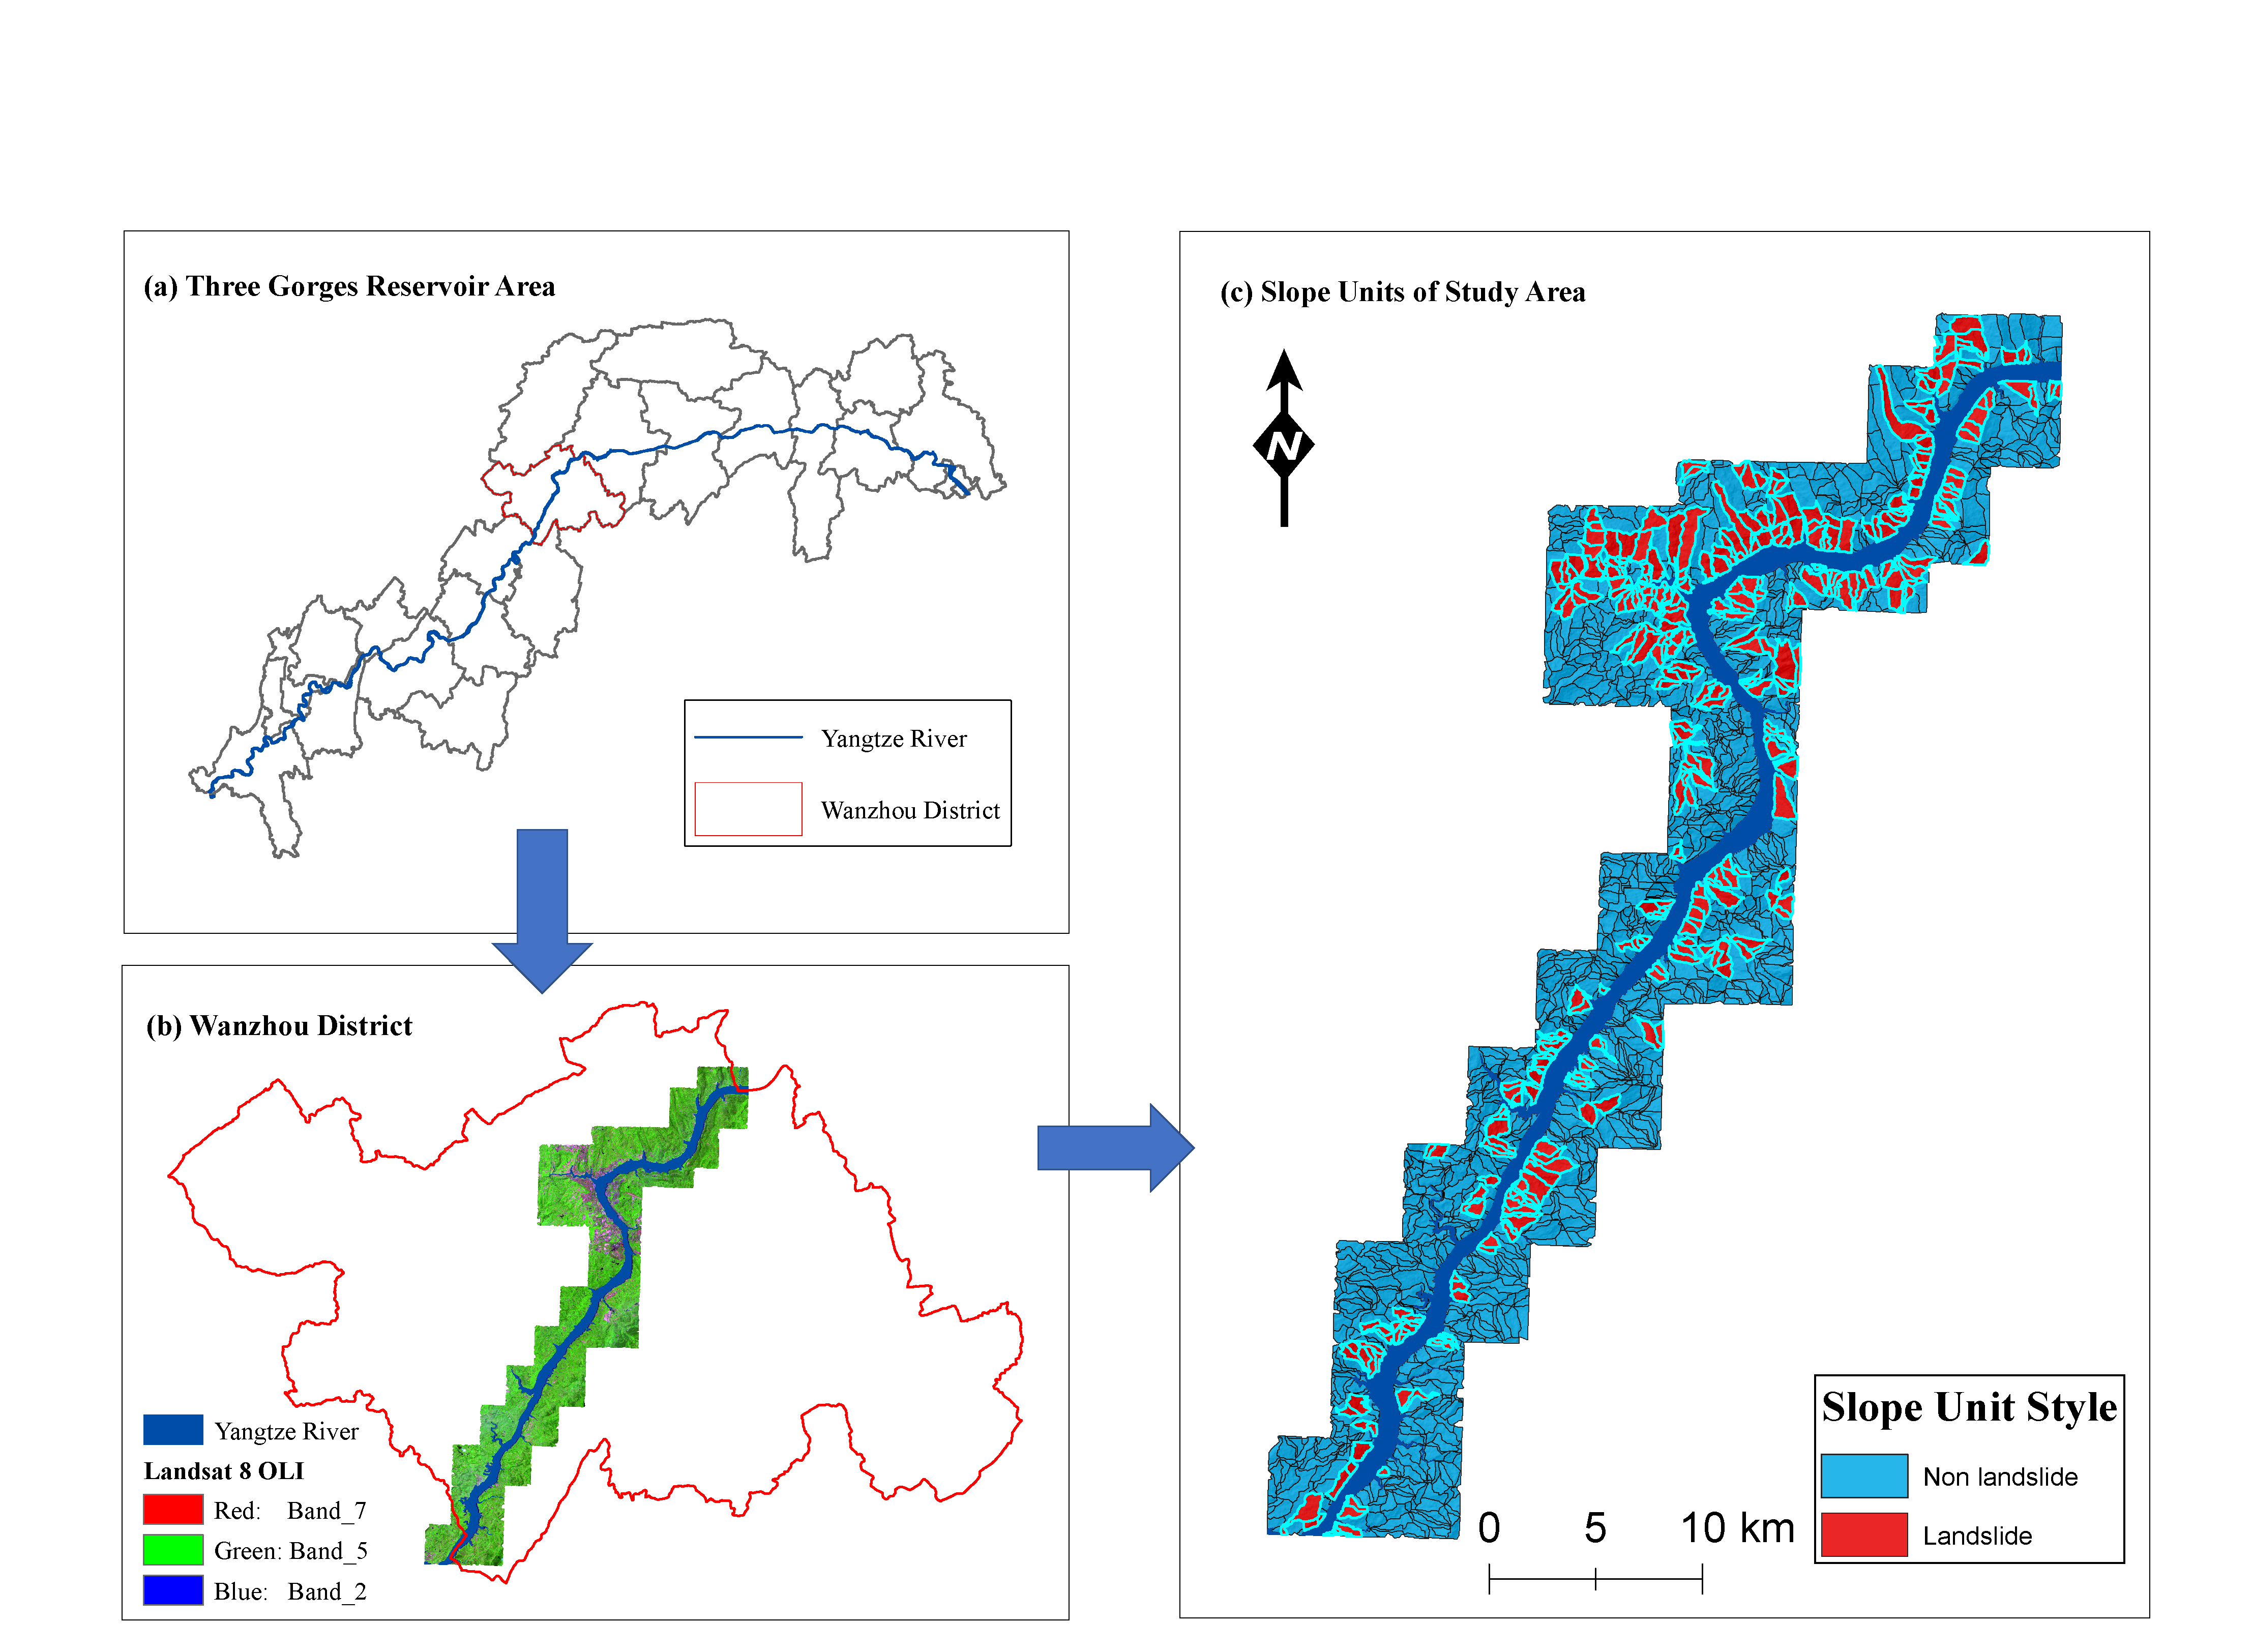
\includegraphics[width=0.9\textwidth]{figs_rev1/Fig_StudyArea.pdf}
    \caption{Study Area. (a)Three Gorges Reservoir area;(b)Wanzhou district;(c)Slope units of study area. Image modified from \cite{Zhang2022}.}
    \label{fig:Figure1}
\end{figure}

\subsection{Study area}
Wanzhou District is located in middle of the Three Gorges Reservoir area, between $107^\circ 55^\prime 22^{\prime \prime}$ - $108^\circ 53^\prime 25^{\prime \prime}$ E and $30^\circ 24^\prime 25^{\prime \prime}$ - $31^\circ 14^\prime 58^{\prime \prime}$ N \citep{Song2018}.
This area has a subtropical humid monsoon climate, with an annual average temperature $17.7^\circ$C and annual precipitation of 1,243 mm.
The study area belongs to the bank section of Wanzhou District, in which the Yangtze River and its tributaries rush \citep{Zhang2022}.
The entire study area is divided into 1,909 slope units, of which 416 are landslide samples, and the rest are non-landslide samples (Fig. \ref{fig:Figure1}).
According to the Digital Elevation Model (DEM) data, the elevation of the study area varies from 21 m to 1,015 m.
Geologically, the lithology is characterized by soft and hard phases, low mechanical strength, and obvious differential weathering, providing favorable environment for the landslides \citep{Zhang2022}.
Tectonically, Wanzhou District is located in the northwest edge of the Sichuan-Hubei-Hunan uplift fold belt, and a lot of tectonic chasms are distributed in NNE or NE direction \citep{Zhang2022}.
Due to these complex geological and climate conditions, the study area has become a famous region for LSP of the Three Gorges Reservoir area. 

\subsection{Data sources}

The data sources used in this study included: 1) $30 \time 30$ m resolution DEM of Aster GDEM; 2) Landsat-8 OLI remote sensing images and Google Earth images; 3) geological maps of 1: 50,000 scale; 4) existing reports and landslide geological survey data; 5) Land use and land cover (LULC) data.
More detailed data can be found from the article of \cite{Zhang2022}.

Slope units could reflect the actual environmental conditions better than grid units, and have definite geological significance \citep{Zhao2021}. 
In this study, we used the hydrological analysis module of ArcGIS to produce the slope units from DEM data. 
Finally, 1,909 slope units were extracted, of which 416 were landslide samples.

A total of 12 landslide factors are used in this article, including slope, aspect, terrain curvature, elevation, rainfall, terrain roughness index (TRI), seismic intensity, distance to the river, lithology, NDVI, NDWI, LULC, etc.
A detailed description of these factors can be found in the article of \cite{Zhang2022}.


\section{Methodology}

\begin{figure}
    \centering
    \includegraphics[width=0.65\textwidth]{figs_rev1/Fig_Workflow.png}
    \caption{Flowchart of the study.}
    \label{fig:Workflow}
\end{figure}

The flowchart of landslide susceptibility prediction for the study area is shown as in Fig. \ref{fig:Workflow}. 
To convert some grid-unit-based landsldie factors (slope, aspect, elevation, etc.) into slope unit, we used the regional statistical tools supported by ArcGIS. 


The factor normalization method is used to eliminate the influence of landslide factor dimension.
The principal component analysis (PCA) method was used for factor dimensionality reduction.
The variance inflation factor (VIF) method was used to carry out multicollinearity analysis of landslide conditioning factors.

To compare the performance of deep learning and ensemble learning in LSP, we used RNN, LSTM, GRU, and AutoML methods to carry out LSP, respectively.
The AutoML was used to find the best model from several ensemble learning models (Adaboost, Xgboost, LightGBM, random forest) quickly and automatically.
ROC/AUC/LPI were used to evaluate the performance of the models.

\subsection{Recurrent neural network (RNN)}

Recurrent neural network (RNN) is a neural network used to process sequence data. 
Compared with the general neural network, it can process the data of the sequence change. 
Every unit is associated with other units in the hidden layer at different time intervals in the RNN method \citep{Wang2020}.
For example, a word will have different meanings because of the different content mentioned above, and RNN can solve this kind of problem well.

\subsection{Long short-term memory neural network (LSTM)}

Long Short-Term Memory Neural Network (LSTM) belongs to a special recurrent neural network (RNN).
The RNN has a directional loop in the hidden layer, and inputs the information in the previous hidden layer to the current hidden layer. 
There is a certain connection between the input data at different time points, rather than being separated from each other. 
But for relatively long sequences, RNN still has the problem of gradient disappearance. 
To solve this problem, LSTM uses a gating mechanism to control the state of the information flow. 
There are three types of gating units in the memory block, which are memory gate, forget gate and output gate. 
The memory gate selectively retains important key information, the forget gate filters unimportant or interference information, and the output gate selects the information output externally.

\subsection{Gate recurrent unit (GRU)}

GRU (Gate Recurrent Unit) is a type of RNN, too. 
Like LSTM, it is also proposed to solve the problems of long-term memory and the disappearance of gradients in backpropagation.
Compared with LSTM, the use of GRU can achieve considerable results, and is easier to train in comparison, which can greatly improve the training efficiency, so it is more inclined to use GRU in many cases.

\subsection{Auto Machine Learning (AutoML) and LightGBM}

Auto Machine Learning (AutoML) was used to select the best ensemble learning models in this article.
AutoML is the end-to-end process automation of applying machine learning to real-world problems.
Starting from the traditional machine learning model, AutoML realizes automation from three aspects: feature engineering, model construction, and hyperparameter optimization, to propose an end-to-end solution.
In this article, we used Microsoft's open source AutoML library -- flaml to select the best ensemble machine learning model from LightGBM, Xgboost, Adaboost, random forest, and finally LightGBM was selected.


The main idea of ensemble learning is to combine multiple weak classifiers (decision tree for LightGBM) to form a strong classifier \citep{Song2018}. 
LightGBM is an improved version of gradient boosting decision tree (GBDT) algorithm proposed by Microsoft \citep{ke2017lightgbm}. 
LightGBM uses a leaf-wise leaf growth strategy with max depth limitation and a histogram-based algorithm to speed up the training process and reduce memory consumption \citep{Gao2021}. 
Therefore, lightgbm has been widely used in processing real world data, which has also been applied to LSP\citep{Song2018,Zhang2022}.

\subsection{Model elevation}
\subsubsection{ROC curve and AUC}

The receiver operator curve (ROC) and the area under the curve (AUC) are widely utilized in evaluating the overall performance of the LSP models \citep{Zhao2021, Gao2021}.
It is a probability curve to show the ability of the classifier to rank the positive samples relative to the negative samples \citep{Gao2021}.
The value of the area under the ROC curve (AUC) is a commonly used indicator to measure the prediction performance, measuring how much the models can distinguish between different classes. 
A higher AUC value always means better model performance \citep{Song2018, Gao2021}.


\subsubsection{Landslide prediction index (LPI)}

By applying the models to the study area, the machine learning models can give the probability of landslide occuring in each slope unit. 
The probability values of the LSP models range from 0 to 1, which are the so-called landslide prediction index values (LPI). 
To get the landslide susceptibility map of each models, the LPI were reclassified as very high, high, moderate, low and very low landslide susceptibility classes with the Natural Breaks method supported by the ArcGIS software. 

\section{Results and discussions}
\subsection{Multicollinearity Analysis of Landslide Factors}

It is of great significance to employ multicollinearity analysis before landslide susceptibility modeling. 
Identifying and selecting appropriate landslide factors is the prerequisite for ensuring the robustness of these models. 
In this study, the variance inflation factor (VIF) was utilized to develop the multicollinearity analysis with the Python programming language (Table 4). 
If the value of VIF exceeds 10, meaning that there are multiple collinearities among variables. 
Results display that all the VIF values of the twelve factors are less than 10, denoting that all the 12 landslide-related factors are appropriate for LSM.

\subsection{Landslide susceptibility mapping results}

LR, LightGBM, RF models, and their weighted models (WLR, WLightGB, WRF) are utilized for landslide susceptibility mapping. 
Twelve landslide contributing factors: elevation, slope, aspect, curvature, distance to the river, NDVI, NDWI, rainfall, seismic intensity, land use, and topographic roughness index (TRI), and lithology were used as the input of these six models. 
The probability values of the six models range from 0 to 1, which are the so-called landslide prediction index values (LPI). 
The LPI values gener-ated by six models were reclassified to develop the landslide susceptibility map with the Natural Breaks method and the ArcGIS software. 
The landslide susceptibility maps (LR \& WLR, LightGBM \& WLightGBM, RF \& WRF) derived from the six models are shown in Figure 5 a–f. 
These landslide susceptibility maps (LSMs) are classified into very low, low, medium, high, and very high susceptibility to landslides. 

The percentages of each category in the six models are illustrated in Figure 6. 
In the LR case, the five landslide susceptibility classes of very low, low, medium, high, and very high covered 41.74\%, 31.55\%, 15.44\%, 8.57\%, and 2.70\% area of the districts, respectively. 
In the LightGBM and RF case, the class of very low area is much higher than those in LR case, while the class of low area is lower than those in LR case, and the classes of medium, high, and very high regions are almost the same as those in LR case. 
The percentages of very low and low classes in LR, LightGBM, and RF cases are higher than those in weighted models, but the percentage of very high and high areas in LR, LightGBM, and RF cases are lower than those in weighted models.

\subsection{Implications for landslide-prone Areas}

The regions with the high and very high landslide susceptibility are mainly distributed on both sides of the river (Figure 5), most likely related to the water level. Wanzhou reservoir area is the hinterland of the Three Gorges Reservoir area with the frequently variable water level. The rising water level of the Yangtze River can lead to the decrease of shear strength of the sliding body through softening and silting the slope (Wang and Qiao, 2013; Gui et al., 2016). In contrast, the drop in the water level produces a much larger hydrodynamic pressure, which increases the sliding force along the direction of underground seepage and then brings about the landslides (Wang and Qiao, 2013; Gui et al., 2016). There is the highest landslide susceptibility at the middle and lower reaches of the river (Figure 5). In addition to lithology, rainfall, and vegetation, the type of land-use is also probably to account for this characteristic. The strata exposed in the Wanzhou reservoir area are mainly Jurassic Shaximiao Formation (J2s) and Suining Formation (J3s) (Zhu et al., 2013). The lithology is off-white feldspathic quartz sand-stone intercalated with purplish-red argillaceous siltstone, purplish-red sandstone, and mudstone. It is easy to form a soft top and hard bottom structural surface because of the difference in weathering speed of mudstone and sandstone, providing an effective structure for the loose accumulation material sliding along the bedrock surface. Wan-zhou District is the center of a rainstorm in eastern Chongqing. According to the Datankou hydrological station's statistics, the average annual precipitation is 1243mm, and the maximum annual rainfall is about 1550mm (Yu et al., 2016; Song et al., 2018). The rainstorm strongly scours the landslide soil, infiltrate into cracks and potential sliding surfaces, resulting in the aggravation of landslide deformation. On the other hand, the rainfall will increase the slope's self-weight, thereby increasing the sliding force of the hill. Therefore, the combination of pore water pressure and soil softening can increase the probability of landslides (Finlay et al., 1997; Dahal et al., 2008). The plant roots have a powerful tensile effect on improving the anti-sliding ability of rock and soil, which anchor the loose weathered layer to the more stable rock and soil layer to prevent them from sliding along the slope. The plant stems and leaves, and litters can intercept and absorbing rainwater, which plays an inhibitory role in slope runoff and rain erosion (Sittadewi and Tejakusuma, 2019). However, the vegetation coverage of the research area is low, having a weak ability to resist landslides. The primary type of land-use in this area is wetland filled with groundwater, which is one of the significant external factors inducing landslide. Groundwater will sharply increase the weight of the rock and soil and reduce the anti-sliding resistance, which leads to the increase of sliding force and slope instability, resulting in landslides. Hence, LSM can be applied to land-use planning and in the prioritizing the management of countermeasures to mitigate potential losses by landslides and also helps the government formulate relevant scien-tific policies according to different susceptibility levels as a means of mitigating land-slides. Moreover, a LSM could also be used to raise public awareness of landslides and then reduce related activities in hazardous areas.

\section{Validation of LSP}

The ROC curves of the six models are shown in Figure 7. 
The AUC values of RNN, GRU, LSTM, LGBM, Xgboost, Catboost, LR, Extra\_tree are 0.611, 0.744, 0.721, 0.972, 0.943, 0.936, 0.988 respectively. 
Based on the AUC results, the ensemble learning methods are generally better than the deep learning methods.
The Extra\_tree model with the highest AUC value (AUC = 0.988) is probably considered to be the best ensemble learning model, and the GRU model (AUC = 0.744) is probably considered to be the best deep learning model.
Landslide events not only reduce the financial losses but also cost human lives. 
A landslide susceptibility map is an essential tool for developing preventive measures in landslide-prone areas. Therefore, many scholars are committed to improving LSM models' performance. 
Recently, machine learning models and ensemble machine learning models had good performance in LSM. 
However, few studies have focused on the class-imbalanced problem, which will lead to poor performance in LSM whether the machine learning or ensemble machine learning models are utilized. 
Thus, we carried out the application of the class-weighted algorithm combined with traditional machine learning (LR) and ensemble machine learning models (LightGBM and RF) to the LSM based on a case study of the Wanzhou section of the Three Gorges Reservoir, China, in the present study. 
The results proved that the weighted methods (WLR, WLightGBM, WRF) are better than unweighted methods (LR, LightGBM, RF), shown as higher AUC, G-mean, and Balanced Accuracy values generally. 
Moreover, the WRF model has much better performance than WLR and WLightGBM models. Although the unweighted models have higher Accuracy value, they are incapable of evaluating landslide susceptibility because their accuracy rates come from the prediction of the negative class (non-landslides) rather than the positive class (landslides). A vital advantage of the weighted models is that the class-weighted algorithm turned the susceptibility evalua-tion problem into a cost-sensitive issue by setting unequal weights for different classes, which improves the performance of LSM, manifesting in higher Recall values. On the other hand, the weighted models (WLR/WLightGBM/WRF) tend to divide more high and very high susceptibility areas than the unweighted models (LR/LightGBM/RF) (Fig 5, 6). Landslide susceptibility map is the basis of landslide risk evaluation. Suppose the high susceptibility area is incorrectly classified as a low susceptibility zone, which may lead to a false judgment on the risk of landslides and then result in considerable threats to the safety of human life and property. Furthermore, the weighted models pay more attention to landslide samples' classification accuracy, which is the actual concern in the landslide susceptibility evaluation. Although every study area has its own unique landslide contributing factors and geological conditions, the weighted models proposed in this paper will provide significant clues for the landslide susceptibility evaluation concerning the imbalanced landslide samples. Regardless, the weighted models still have several disadvantages. 
For instance, the cost matrix should be processed before classification using weighted models, which is affected by the processing method and is time-consuming. Moreover, a high-resolution DEM for the study area is not freely available, resulting in the poor performance of weighted models. If high-resolution DEM were utilized for extracting landslide-related parameters, these weighted models could achieve better results. 

\section{Conclusions}

In the prediction of landslide susceptibility, the choice of method has a great influence on the accuracy of the evaluation results. 
Deep learning methods have also been increasingly applied to the evaluation of landslide susceptibility. 
However, little research has explored whether deep learning methods are always appropriate. 
In this article, we compared the deep learning method and the ensemble learning method on the slope-unit-based landslide susceptibility evaluation, and found that the ensemble learning method is more effective. 
It is not advisable to blindly choose deep learning methods for landslide susceptibility evaluation modeling, and it is necessary to consider the scale of landslide samples.

\section{Acknowledgments}

The authors would like to acknowledge Prof. Chong Xu for helpful discussions. 
This research was funded by Project Digital frequency spectrum analysis and mineralization precise prediction for continental su-pergene U-Re (No. 41872243), East China University of Technology Doctoral Research Startup Fund (No. DHBK2019218), Jiangxi Provincial Nuclear and Geoscience Data Science and System Engineering Technology Research Center (No.JETRCNGDSS202002), National Natural Science Foundation of China (No. 41807297), and Jiangxi Engineering Laboratory on Radioactive Geoscience and Big Data Technology (No. JELRGBDT202004).

\newpage

\textbf{Code availability section}

ArcGIS 10.8 and QGIS 3.16 were used to extract landslide factors, visualize landslide factors and export result maps.

The source codes are available for downloading at the link:
https://github.com/songyingxu/LspModelsForCageo


\bibliographystyle{cas-model2-names}
\bibliography{bibliography} 

\end{document}

